\refstepcounter{chapter}
\addcontentsline{toc}{chapter}{INHALTSVERZEIGNIS}

\thispagestyle{coverpage}

\begin{titlepage}
    \thispagestyle{coverpage}

    \vspace*{0cm}

    {\sffamily

        \noindent
        \begin{tabularx}{\textwidth}{X r}
            
\includegraphics[height=1.5cm]{maho-logo.png} &
            {\Huge \textbf{Operator's Manual}} \\
            \multicolumn{2}{l}{\rule{\textwidth}{0.4mm}} \\
            & {\normalsize Nr. 76.34521}
        \end{tabularx}

        \centering
        \vspace{2cm}

        {\fontsize{60pt}{62pt} \bfseries MH400E}\\[1cm]

        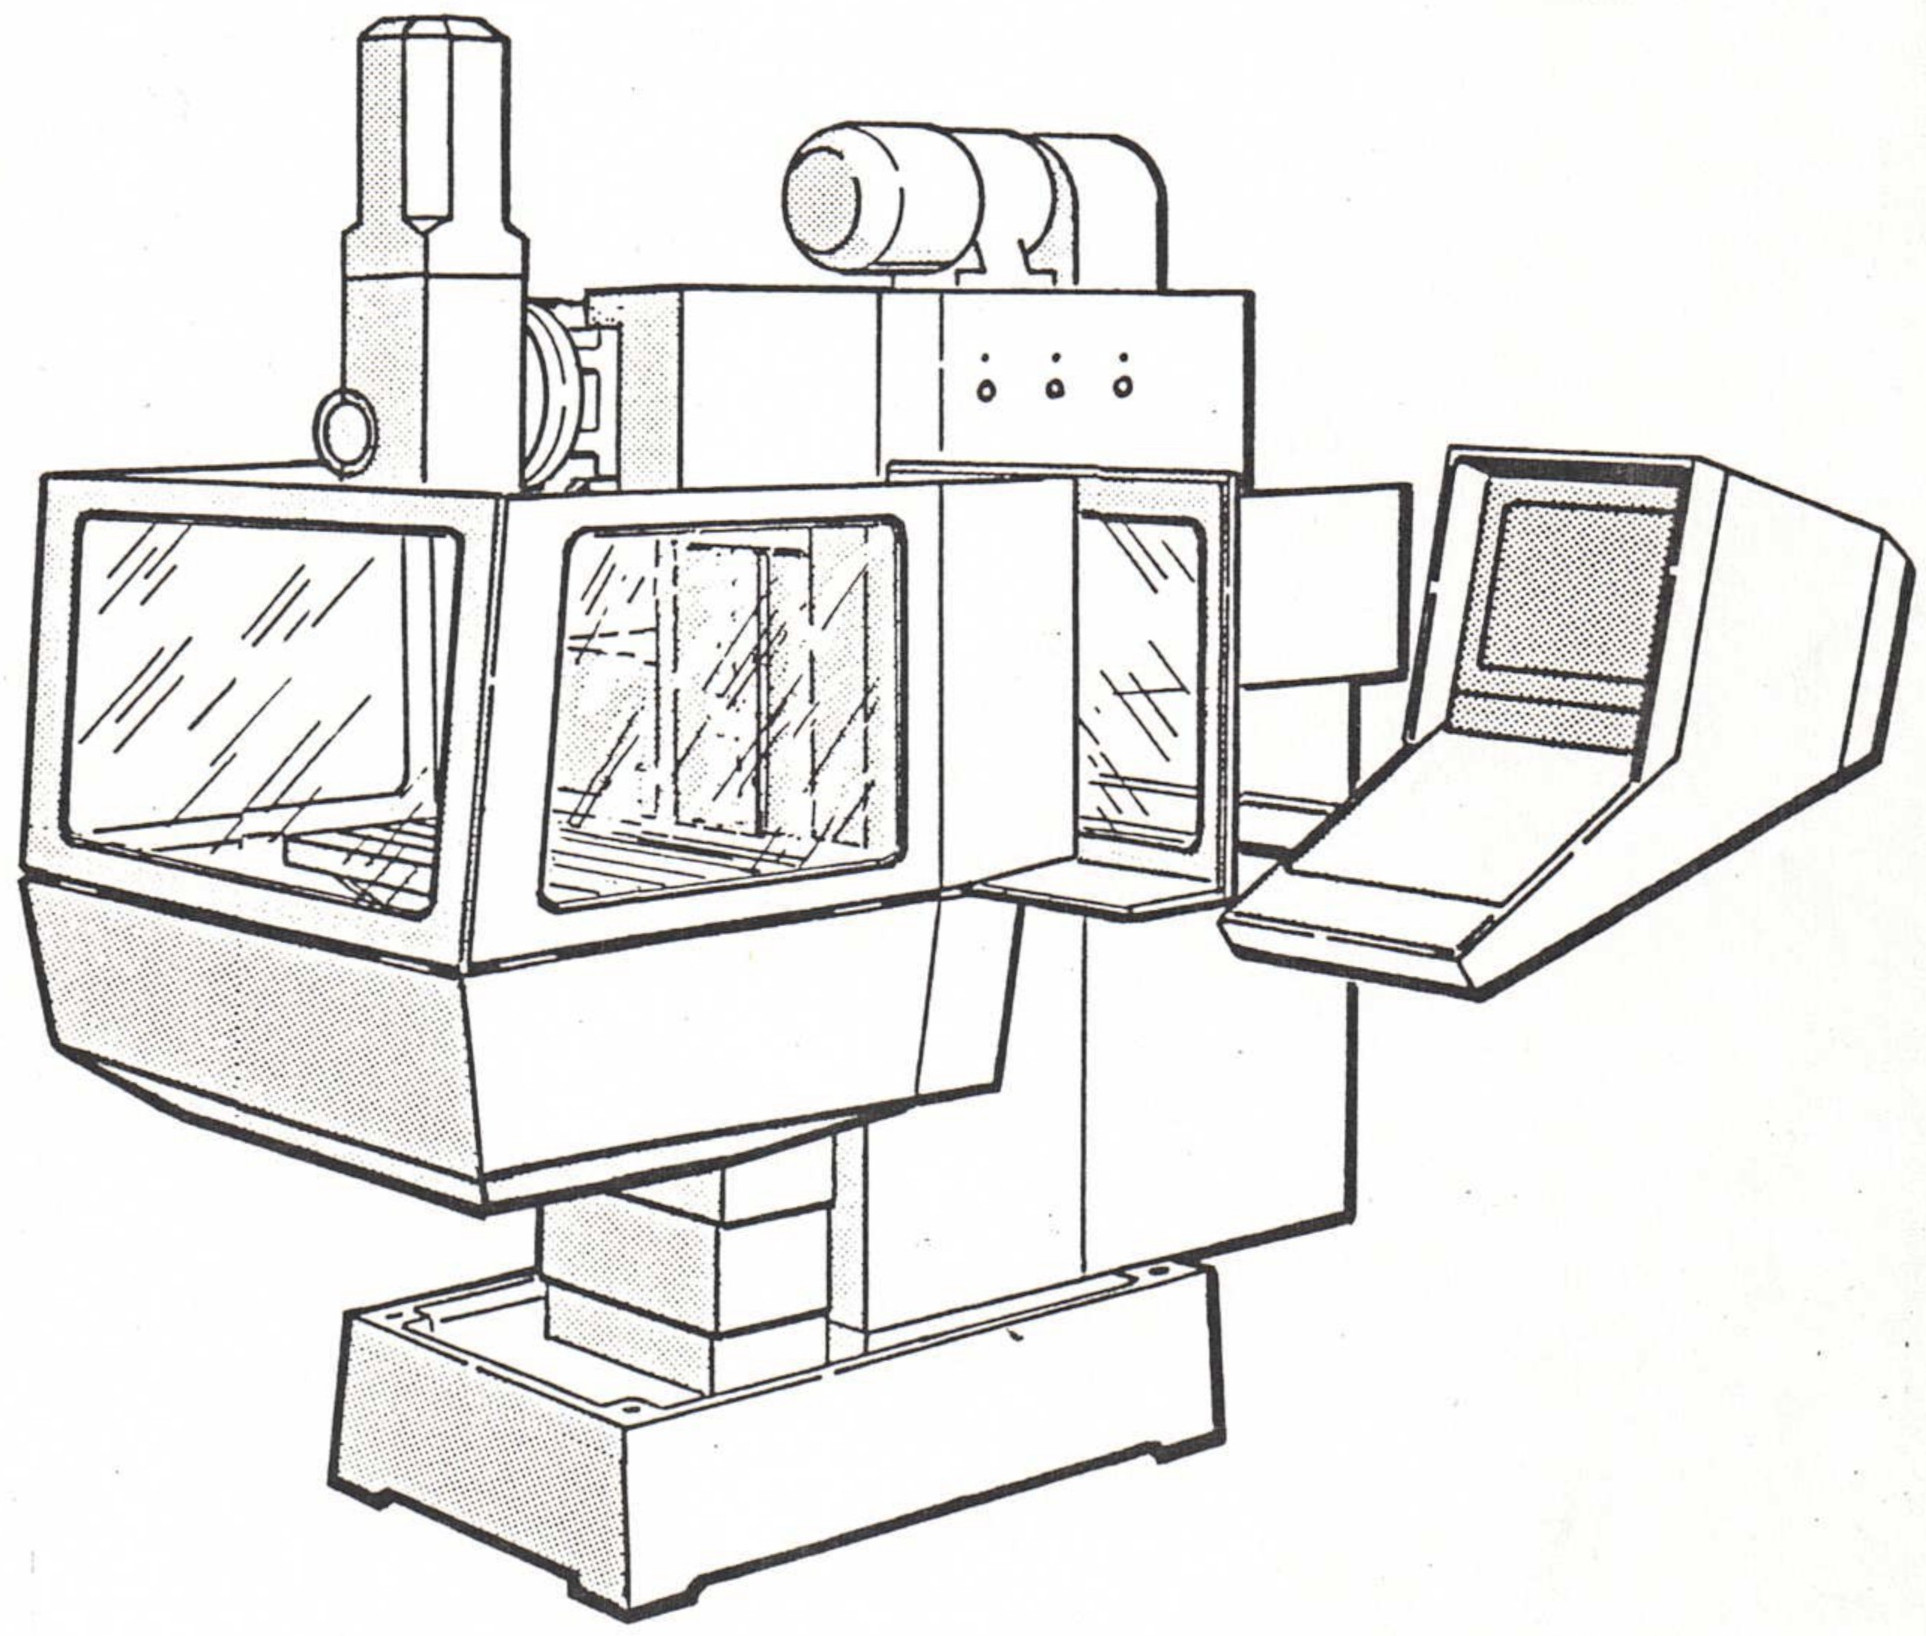
\includegraphics[width=0.9\textwidth]{chapter0/cover-image.jpg} 

        \vfill

         \noindent
         \begin{center}
             \parbox{\textwidth}{\centering {\Huge \textbf{Operation - Maintenance - Repair}}}
         \end{center}
    }
\end{titlepage}

\clearpage % Move to the next page and resume normal styling
\pagestyle{fancy} % Re-enable the default layout

\setsectiontitle{To our customers}
\setcounter{chapter}{0}
\setcounter{section}{0}

This operator's manual contains the essential information required for the proper operation and maintenance of your MAHO machine tool. It belongs in the hands of the operating and maintenance personnel.

The present operator's manual includes the separate operating instructions for CNC 432/10 graphics, the programming instructions for CNC 432 of the control unit, the programming manual for the \enquote{Geometry Package}, and the folder \enquote{Assembly Drawings and Parts Lists}.

Tax-specific details are listed \textbf{only} in the operating manual for CNC 432/10 graphics and should be referenced there.

The machine may only be put into operation after the operating and maintenance personnel have carefully read the operator's manual and have thoroughly\\ familiarized themselves with all details.

Operation and maintenance of the machine must be carried out in accordance with the instructions provided in this operator's manual.

\notebox{NOTE}{\textbf{We assume no liability for damages resulting from failure to follow these instructions or from improper handling.}}

If malfunctions occur that cannot be resolved independently, the cause of the malfunction should be determined using the operator's manual before \\contacting the appropriate MAHO representative or the MAHO company.

This operator's manual is designed to help you complete your machining tasks efficiently. We are confident that the delivered MAHO machine tool will fully meet your expectations. \\[1cm]

\noindent
\textbf{\textcopyright\ Copyright} \\[0.2cm]

This technical manual may \textbf{not}, even in part, be reproduced or made accessible to third parties without the express permission of the publisher.

\newpage

\subsection{Page Numbering}

The pages of this manual are numbered sequentially within each chapter \\according to sections. The page numbers are displayed in the upper right corner and are structured so that the page number follows the section number.

\textbf{EXAMPLE}: \texttt{3.20-3}, means Chapter 3, Section 20, Page 3.

If expansions occur within a section, these are numbered using the page number of the previous page followed by the numbers 1, 2, 3, etc., separated by a period.

\textbf{EXAMPLE}: \texttt{3.20-3.1}, means Chapter 3, Section 20, Page 3, Supplementary Page 1.

Figures and tables are not separately numbered.

The position numbers in the figures refer to the content of the section and can span 2-3 figures.

If positions of a figure are referenced in the text, they are placed within parentheses \texttt{()}.

\subsection{Notices in this Manual}

The following notices are used in this manual:

\notebox{NOTICE}{Applies to technical details that the user must observe.}

\notebox{CAUTION}{Applies to work or operational procedures that must be followed precisely to prevent damage or destruction of the system.}

\notebox{WARNING}{Applies to work or operational procedures that must be followed precisely to prevent hazards to personnel. This also includes \textbf{CAUTION}.}

\subsection{Cross-References}

To avoid redundant descriptions, content-related connections are established in this manual using cross-references.

\textbf{EXAMPLE}:
\begin{quote}
\noindent \hspace{-0.25cm} .... according to instructions .... \\
\hspace{1.3cm} .... see Sheet/Page ....
\end{quote}

\subsection{Location Definition}

The designations front, back, left, right, top, and bottom are based on the perspective from the spindle head looking toward the workpiece.
